\documentclass[utf8]{frontiersSCNS}
\usepackage{gensymb}
\usepackage{url,hyperref,lineno,microtype,subcaption}
\usepackage[onehalfspacing]{setspace}

\linenumbers
\usepackage{wasysym} % provides \DH, \dh, \Thorn, \thorn
% Leave a blank\usepackage{amsmath}
%\DeclareMathOperator{\sign}{sign} line between paragraphs instead of using \\

\usepackage{booktabs}
\usepackage{multirow}
\usepackage{siunitx} %for SI units
\usepackage{lscape} % for landscape table

\def\keyFont{\fontsize{8}{11}\helveticabold }
\def\firstAuthorLast{Balasubramanian {et~al.}} %use et al only if is more than 1 author
\def\Authors{Suryanarayanan Balasubramanian\,$^{1}$, Roger Waser\,$^{2}$, Martin Hoelzle\,$^{1}$}
\def\Address{$^{1}$University of Fribourg, Department of Geosciences, Fribourg, Switzerland $^{2}$University of
Applied Sciences and Arts, Luzern, Switzerland} \def\corrAuthor{Suryanarayanan Balasubramanian}

\def\corrEmail{suryanarayanan.balasubramanian@unifr.ch}


\begin{document}
\onecolumn
\firstpage{1}

\title[Scheduling AIR fountains]{Fountain scheduling recommendations to improve water use efficiency of artificial ice reservoir (Icestupas)}

\author[\firstAuthorLast ]{\Authors}
\address{}
\correspondance{}

\extraAuth{}

\maketitle

\begin{abstract}
  To construct artificial ice reservoirs (AIRs) with limited water resources requires a high water use
  efficiency (WUE). This can be achieved by the precise scheduling of the fountain water spray taking into
  account the AIRs response to weather conditions. We solve the corresponding optimization problem, i.e. finding
  the ideal discharge rate for maximum WUE by two approaches differing in operation costs which offer
  straightforward application facilities . The automation software uses a simplified equation with 6
  coefficients that captures the influence of temperature, humidity, wind and solar radiation variations on the
  freezing rate. Historical meteorological data of the site is required to calculate these 6 coefficients. The
  automated AIR had a WUE three times more than the manual AIR. These results support the use of the model in
  practice. 

  \tiny \keyFont{ \section{Keywords:} icestupa, water storage, climate change adaptation,
  geoengineering, nature based solution} 
\end{abstract}

\section{Introduction}
Artificial Ice Reservoirs (AIRs) have recently received much attention in the light of increasing users,
especially in semi-arid and arid mountain regions facing limited water availability and at the same time
increased water needs. However, their water use efficiency (WUE) is very poor. 

Fountain scheduling methods are one option for reducing watering volumes for AIR construction systems and, at
the same time, increase WUE. The goal of fountain scheduling is to make the most efficient use of water by
spraying the right amount of water at the right time, making sure water is available when the AIR surface can
freeze it. Scheduling maximizes AIR WUE by minimizing fountain waste water.  

Proper fountain scheduling requires answers to two questions: (a) When should the water be turned on and off?
(b) How much water should be sprayed? Knowledge of surface freezing rates is important for answering these
questions. Surface freezing rates can be calculated by means of two different approaches: physical
energy-balance models and empirical models. The former may be defined as a model in which each of the relevant
energy fluxes at the AIR surface is computed from physically based calculations using direct measurements of the
necessary meteorological variables, and the freezing rate is calculated as the sum of the individual fluxes
scaled with the AIR surface area during the accumulation period. The latter may be defined as a model in which
the freezing rate is calculated from an empirical formula in which air temperature, relative humidity and wind
speed are the measured input variable, although additional input variables, such as incoming solar radiation,
may be incorporated through parametrizations based on time and location. Empirical models have been widely used
for both glaciological and hydrological applications due to their parsimony in data requirement in comparison
with the more sophisticated energy-balance models.

Since this technology is currently being used by subsistence farmers, we also need to be mindful of the
maintenance and implementation costs. We propose two different methods of fountain scheduling based on operation
costs that can be classified as static or dynamic. According to the static approach, the total amount of water
for AIR construction is allocated without specifying its temporal distribution along the accumulation period. By
contrast, in the dynamic approach water is allocated at specific time steps along the accumulation period in
order to achieve even higher WUE.

Both the approaches use a fountain and pipeline system with minimal manual intervention. The dynamic approach is
better suited for locations where the diurnal and seasonal variations in the weather conditions are significant.
In such cases, the real-time adjustments of the automated discharge rate make efficient fountain scheduling
possible. The static approach is better suited for other locations or for users who cannot afford the additional
cost of the automation system.

\section{Fountain scheduling software}

The objective of the automation software is to estimate the freezing rate given minimal weather, fountain and
location information. For this purpose, we construct a simplified model using components of the energy balance
model used in \cite{balasubramanianInfluenceMeteorologicalConditions2022} and \cite{oerlemansBriefCommunicationGrowth2021}. 

The freezing rate of the AIR can be represented as: 

\begin{equation}
	 \frac{\Delta M_{freeze}}{\Delta t}  = (q_{SW} + q_{LW} + q_{L} + q_{S} + q_{F} + q_{G}) * A_{cone}
	\label{eqn:freeze}
\end{equation}

We simplify the estimation of each of the energy flux components using assumptions that underestimate the
associated freezing rate to optimise for WUE. Further description of our assumptions are described in the
Appendix. Below, we summarise the list of assumptions used:

\begin{itemize}

  \item Surface Area $A_{cone}$ : The area of the conical AIR is approximated to the area of its circular base
    produced through the fountain spray radius $r_F$. This assumption is derived from
    \cite{oerlemansBriefCommunicationGrowth2021} model and underestimates the surface area of the AIR during
    the accumulation period and thereby underestimates the freezing rate.

  \item Shortwave Radiation $q_{SW}$: The direct and diffuse components of shortwave radiation are estimated from the coordinates,
    altitude and time using the PVLIB python package described in \cite{holmgrenPvlibPythonPython2018} . The algorithm used to
    estimate the clear-sky global radiation is described in and the algorithm used to estimate the diffuse part
    of the global radiation is described in . Furthermore, the solar area fraction is also approximated by
    assuming $h_{cone} = r_{cone} = r_{F}$ and the albedo is assumed to be equal to ice albedo (0.25). These
    assumptions underestimate the freezing rate.

  \item Longwave Radiation $q_{LW}$: We assume $T_{ice} = 0 \degree C$. This assumption overestimates $q_{LW}$ and thereby
    underestimates the freezing rate.

  \item Turbulent fluxes ($q_{L}$ and $q_{S}$): The software estimates the pressure using the altitude of the location and ignores
    the $\mu_{cone}$ parameter thereby underestimating the turbulent fluxes.

  \item $q_{F}$ and $q_{G}$: We ignore the influence of fountain water heat flux and the ground heat flux.

\end{itemize}

Using the above simplifications, we can now approximate $q_{LW}$, $q_{L}$ and $q_{S}$ using just temperature,
relative humidity, wind speed and altitude. 

\begin{subequations}
	\begin{align}
		\label{eqn:T}
  (\frac{q_{LW} + q_{S}}{L_F} + \frac{q_L}{L_V}) \cdot \Delta t & = a \cdot T_a + b \cdot RH + c \cdot v_a +
  d \cdot alt + e \\
		\label{eqn:sun}
  \frac{q_{SW}}{L_F}\cdot \Delta t & = G(time, coords, alt) \\
		\label{eqn:auto}
  \frac{\Delta M_{freeze}}{\Delta t} &= (G(time, coords, alt) + f(T_a, RH, v_a, alt)) \cdot \pi \cdot r_F^2 
	\end{align}
\end{subequations}

where $G$ is the solar radiation flux function described in the Appendix.


\begin{table}[ht]
\centering
\caption{}
\label{tab:my-table}
\begin{tabular}{@{}lllllll@{}}
\toprule
Coefficients of & $T_a$ & $RH$ & $v_a$ & $alt [km]$  & $constant$ \\ \midrule
Value           & $\num{-5.6 e-3}$     & $\num{-3.2 e-4}$ & $\num{4.7 e-3}$ & $\num{-3.5 e-3}$  & $\num{5.2 e-3}$
                \\ \bottomrule
\end{tabular}
\end{table}

\section{Dynamic fountain scheduling prototype}

\begin{figure}[ht]
	\begin{center}
		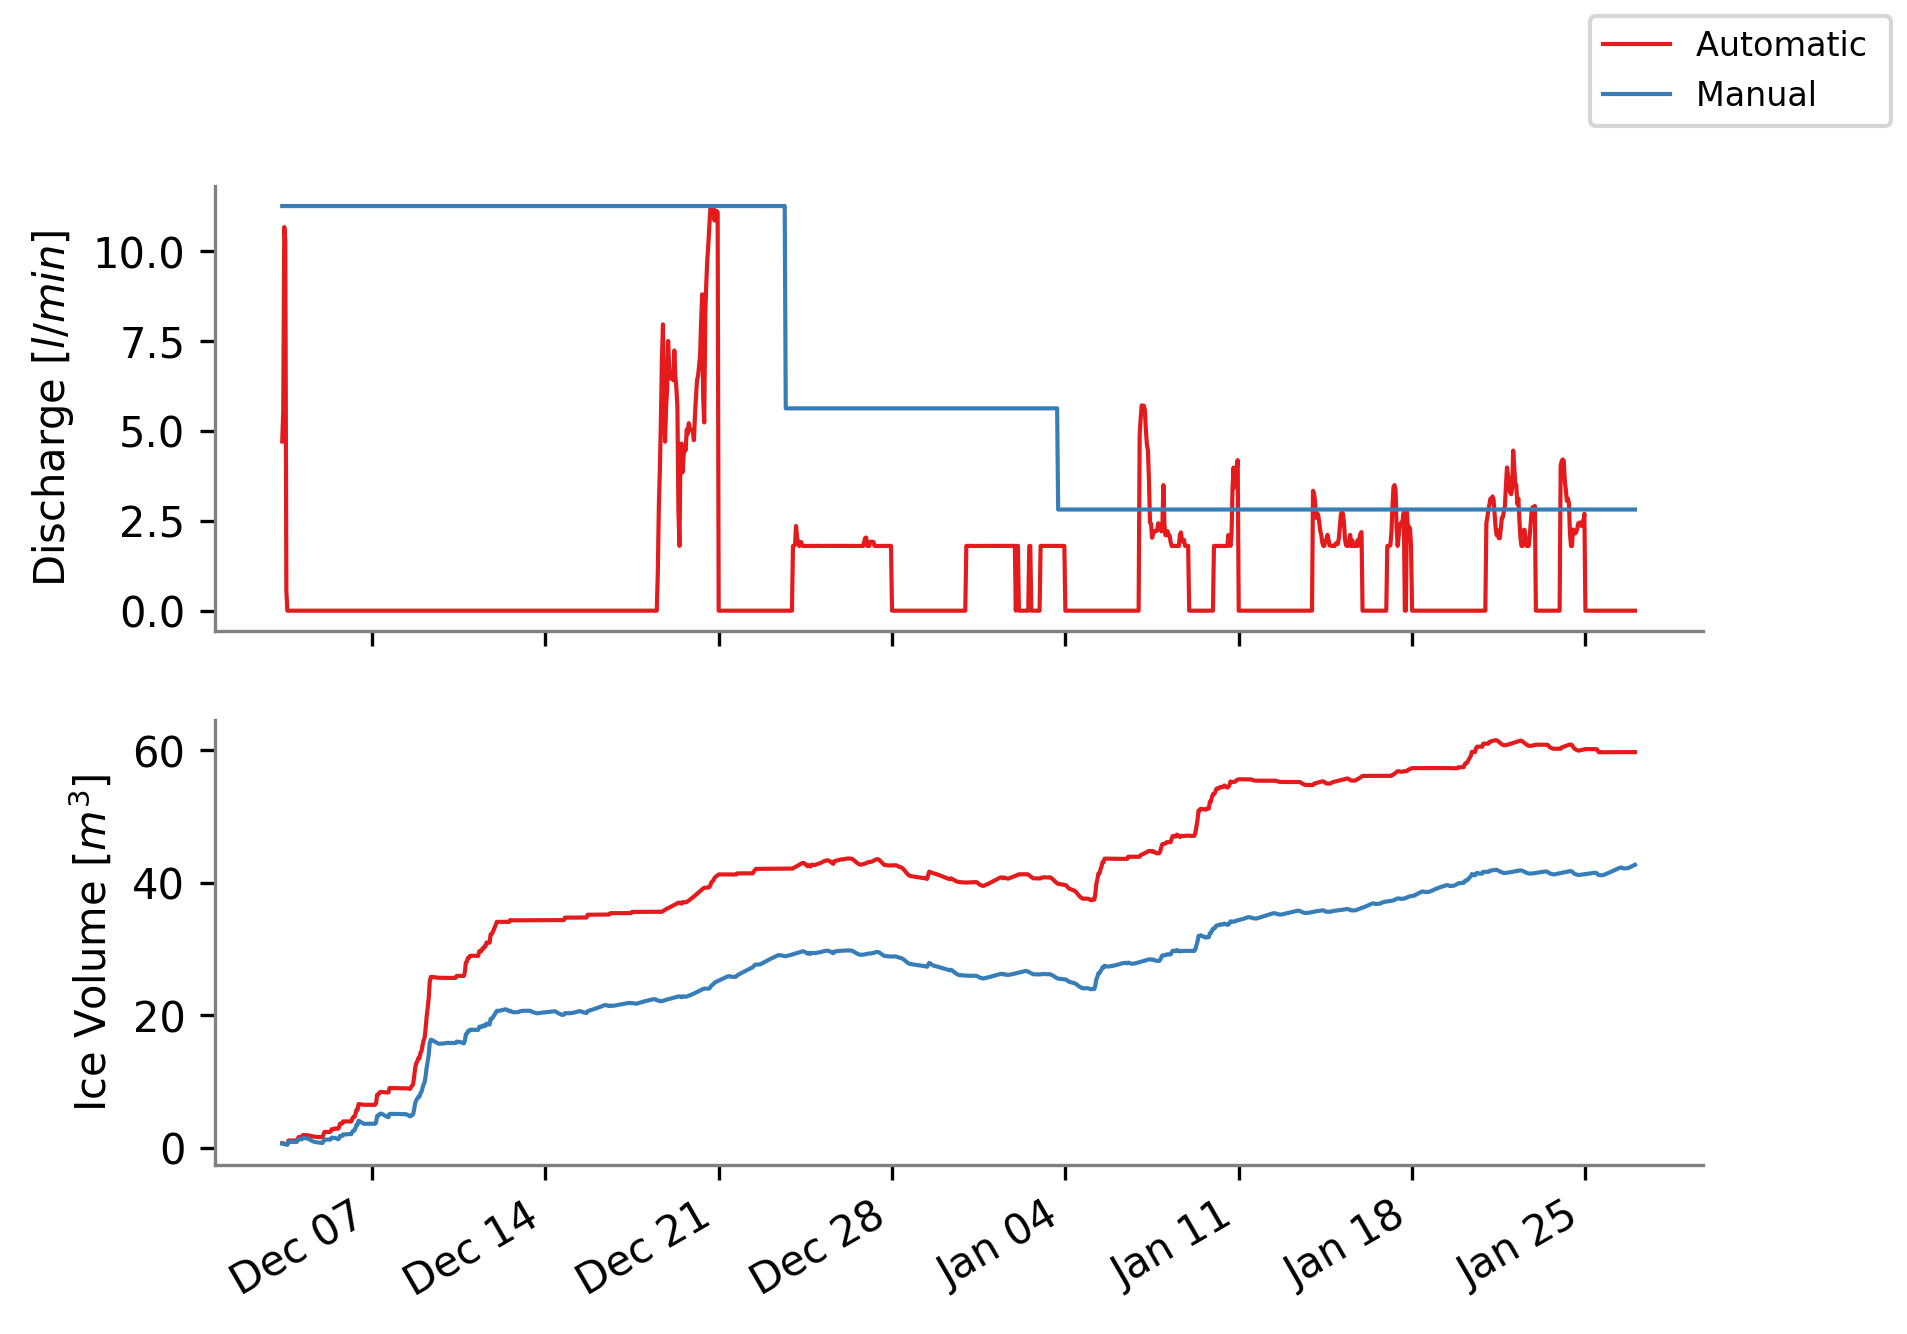
\includegraphics[width=\linewidth]{Figures/autovsmanual.png}
	\end{center}
	\caption{Comparison of discharge and ice volume between AIRs produced by dynamic and static fountains. }
	\label{fig:old_icestupa}
\end{figure}

\section{Recommendations}
\subsection{Static fountain scheduling}
\subsection{Dynamic fountain scheduling}

The automation hardware consists of a weather station, flowmeter, control valve, drain valves, air valves,
fountain, pipeline and a logger. The logger feeds the weather station data to the automation equation and
informs the expected freezing rate to the flowmeter. The flowmeter adjusts the control valve to match the
discharge rate recommendation of the logger. In case this discharge recommendation is below the critical
discharge rate of the the fountain, the drain and air valves empty the water in the pipeline to prevent any
freezing events. Here the critical discharge rate is defined as the discharge rate below which the fountain
pipeline can freeze.

\subsection{Fountain height and spray radius}


\section{Discussion}

\subsection{Limited and unlimited water availability}

\subsection{Fountain vs weather influence}

\subsection{Ideal fountains and locations for AIR construction}

\section{Conclusions}


\section{Appendix}

The area of the conical AIR is approximated to the area of its circular base produced through the fountain spray
radius $r_F$. Therefore, the surface area can be determined using

\begin{equation} A_{cone} =\pi \cdot r_{F}^2 \label{eq:Area} \end{equation}

Admittedly, this assumption underestimates the surface area of the AIR during the accumulation period and
thereby underestimates the freezing rate.

We approximate the energy balance at the surface of an AIR by a one-dimensional description of energy fluxes as
used in \cite{balasubramanianInfluenceMeteorologicalConditions2022}:


Upward and downward fluxes relative to the ice surface are positive and negative, respectively. The first
term represents the energy change used for freezing the fountain water and melting the ice respectively.
$q_{SW}$ is the net shortwave radiation; $q_{LW}$ is the net longwave radiation; $q_{L}$ and $q_{S}$ are the
turbulent latent and sensible heat fluxes. 

The software assumes $T_{ice} = 0 \degree C$ and therefore ignores the temperature change flux $q_{T}$, fountain
heat flux $q_{F}$ and ground heat flux $q_{G}$. All these assumptions overestimate the freezing rate.

Furthermore, we the rest of the energy balance components based on their air temperature and solar
radiation dependence. Namely, $q_{LW}$, $q_{L}$ and $q_{S}$ contribute to temperature induced freeze rate and
$q_{SW}$ contributes to solar radiation induced melt rate during the accumulation period.  Particularly,

For the static method, we only need to determine the night freezing rates whereas for the dynamic approach we
also need to account for the day melt during the accumulation period.

\subsection{Net Longwave radiation \texorpdfstring{$q_{LW}$}{Lg}} \label{sec:LW}
The net longwave radiation $q_{LW}$ is determined as follows:

\begin{equation}
	q_{LW}= \sigma \cdot \epsilon_a \cdot {(T_a+ 273.15)}^4 -\sigma \cdot \epsilon_{ice} \cdot {(T_{ice}+ 273.15)}^4
	\label{eqn:LW}
\end{equation}

where $T_a$ represents the measured air temperature, $\epsilon_a$ denotes the atmospheric emissivity $T_{ice}$
is the modelled surface temperature given in [$\degree C$], $\sigma=5.67\cdot10^{-8}\,Jm^{-2}s^{-1}K^{-4}$ is
the Stefan-Boltzmann constant and $\epsilon_{ice}$ is the corresponding emissivity value for the Icestupa
surface (0.97).

We approximate the atmospheric emissivity $\epsilon_a$ ,
considering air temperature and vapor pressure (Eqn. \ref{eqn:atm_e}). The vapor pressure of air over water and
ice was obtained using Eqn. \ref{eqn:vp}.  The expression defined in \cite{brutsaertDerivableFormulaLongwave1975} for clear skies
(first term in equation \ref{eqn:atm_e}) is extended with the correction for cloudy skies after
\cite{brutsaertEvaporationAtmosphereTheory1982} as follows:

\begin{equation}
	\epsilon_a=1.24 \cdot (\frac{p_{v,w}}{(T_a+273.15)})^{1/7}\cdot(1+0.22\cdot{cld}^2) \label{eqn:atm_e}
\end{equation}

with a cloudiness index $cld$, ranging from 0 for clear skies to 1 for complete overcast skies. 

The software assumes $T_{ice} = 0 \degree C$. This assumption overestimates $q_{LW}$ and thereby underestimates
the freezing rate.

\subsection{Turbulent fluxes} \label{sec:Qs}

The turbulent sensible $q_{S}$ and latent heat $q_{L}$ fluxes are computed with the following expressions
proposed by \cite{garrattAtmosphericBoundaryLayer1992}:

\begin{equation}
	q_{S}= c_{a} \cdot \rho_{a} \cdot p_{a}/p_{0,a} \cdot \frac{\kappa^2 \cdot v_a \cdot
		(T_a-T_{ice})}{{(\ln{\frac{h_{AWS}}{z_{0}}})}^2}
	\label{eqn:qs}
\end{equation}

\begin{equation}
	q_{L}= 0.623 \cdot L_s \cdot \rho_{a}/p_{0,a} \cdot \frac{\kappa^2 \cdot
	v_a(p_{v,w}-p_{v,ice})}{{(\ln{\frac{h_{AWS}}{z_{0}}})}^2}
\end{equation}

where $h_{AWS}$ is the measurement height above the ground surface of the AWS (around $2\,m$ for all sites),
$v_a$ is the wind speed in [$m\,s^{-1}$], $c_a$ is the specific heat of air at constant pressure (1010 J
$kg^{-1} K^{-1}$), $\rho_{a}$ is the air density at standard sea level (1.29 $kg m^{-3}$), $p_{0,a}$ is the air
pressure at standard sea level (1013 $hPa$), $p_{a}$ is the measured air pressure, $\kappa$ is the von Karman
constant (0.4), $z_{0}$ is the surface roughness (3 $mm$) and $L_s$ is the heat of sublimation (2848
$kJ\,kg^{-1}$).  The vapor pressure of air with respect to water ($p_{v,w}$) and with respect to ice
($p_{v,ice}$) was obtained using the formulation given in \cite{huangSimpleAccurateFormula2018} :

\begin{equation}
	\begin{split}
		p_{v,w}&=e^{\frac{(34.494 - \frac{4924.99}{T_{a} + 237.1})}{(T_a + 105)^{1.57} \cdot 100}} \cdot \frac{RH}{100} \\
		p_{v,ice}&=e^{\frac{(43.494 - \frac{6545.89}{T_{ice} + 278})}{(T_{ice} + 868)^{2} \cdot 100}} \\
	\end{split} \label{eqn:vp}
\end{equation}

The software ignores the $\mu_{cone}$ parameter thereby underestimating the turbulent fluxes. Since turbulent
fluxes impact both the freezing and the melting rates, this assumption may not underestimate freezing rates.

\subsection{Net shortwave radiation \texorpdfstring{$q_{SW}$}{Lg}}
\label{sec:SW}

The net shortwave radiation $q_{SW}$ is computed as follows:

\begin{equation} q_{SW} = (1- \alpha_{ice}) \cdot ( SW_{direct} \cdot f_{cone} + SW_{diffuse})
\label{eqn:SW} \end{equation}

where $\alpha_{ice}$ is the bare ice albedo value (0.25); $SW_{direct}$ is the direct shortwave radiation. The
global shortwave radiation used is modelled using the parametrisation proposed by \cite{woolfComputationSolarElevation1968}.

The solar area fraction $f_{cone}$ of the ice structure exposed to the direct shortwave radiation depends on the
shape considered. Using the solar elevation angle $\theta_{sun}$, the solar beam can be considered to have a
vertical component, impinging on the horizontal surface (semicircular base of the AIR), and a horizontal
component impinging on the vertical cross section (a triangle). The solar elevation angle $\theta_{sun}$ used is
modelled using the parametrisation proposed by \cite{woolfComputationSolarElevation1968}. Here we overestimate the impact of direct
solar radiation by assuming $h_{cone} = r_{cone} = r_{F}$. Accordingly, $f_{cone}$ is determined as follows:

\begin{equation}
	\begin{split}
		f_{cone}& =\frac{ cos \theta_{sun} + \pi \cdot sin \theta_{sun} }{2\sqrt{2} \cdot \pi }\\
	\end{split}
	\label{ eqn:f_{cone}}
\end{equation}

The software ignores the variations in the albedo and assumes it to be equal to that of ice to simplify the
model. This assumption overestimates the solar radiation absorption thereby underestimating the freezing rate.

\bibliographystyle{frontiersinSCNS_ENG_HUMS} \bibliography{zot_refs}

\end{document}

% \begin{landscape}
% \begin{table}[]
% \centering
% \caption{}
% \label{tab:my-table}
% \begin{tabular}{@{}lllll@{}}
% \toprule
% \textbf{Module name} & \textbf{Symbol} & \textbf{Full eqn} & \textbf{Simplified eqn} & \textbf{Assumptions} \\ \midrule
% \multicolumn{1}{|l}{Surface Area}        & $A_{cone}$ &  & \pi \cdot r_{F}^2 & \multicolumn{1}{l|}{} \\ \midrule
% \multicolumn{1}{|l}{Shortwave Radiation} & $q_{SW}$ &  & (1- \alpha_{ice}) \cdot ( (1- cld) \cdot SW_{global} \cdot f_{cone} + cld \cdot SW_{global}) & \multicolumn{1}{l|}{} \\ \midrule
% \multicolumn{1}{|l}{Longwave Radiation}  & $q_{LW}$ &  & \sigma \cdot \epsilon_a \cdot {(T_a+ 273.15)}^4 -\sigma \cdot \epsilon_{ice} \cdot {273.15}^4 & \multicolumn{1}{l|}{} \\ \midrule
% \multicolumn{1}{|l}{Sensible Heat}       & $q_{S}$ &  &  & \multicolumn{1}{l|}{} \\ \midrule
% \multicolumn{1}{|l}{Latent Heat}         & $q_{L}$ &  &  & \multicolumn{1}{l|}{} \\ \bottomrule
% \multicolumn{1}{|l}{Temperature heat flux} & $q_{T}$ &  & 0 & \multicolumn{1}{l|}{} \\ \bottomrule
% \multicolumn{1}{|l}{Fountain discharge heat flux} & $q_{F}$ &  & 0 & \multicolumn{1}{l|}{} \\ \bottomrule
% \multicolumn{1}{|l}{Ground heat flux}    & $q_{G}$ &  & 0 & \multicolumn{1}{l|}{} \\ \bottomrule
% \end{tabular}
% \end{table}
% \end{landscape}
